\section{TeraHeap Design}
\subsection{Overview}
\label{sec:over}

The key idea of \teraheapName{}, as shown in Figure~\ref{fig:teraheap}, is to
extend the JVM to use a second, high-capacity managed heap (H2) over a
fast storage device that coexists with the regular managed heap (H1).
Unlike DRAM-backed H1, H2 is memory-mapped over a storage device,
allowing direct access to deserialized objects without \teraheapSD.
Memory-mapped I/O eliminates the need to use a custom reference lookup
mechanism in the JVM to identify objects on the device, as the OS
virtual memory mechanism performs this translation.
\teraheapName{} manages the two heaps differently and hides their
heterogeneity, providing to big data applications the abstraction of a
single managed heap.

Although \teraheapName{} is agnostic to the specific device that backs H2, the
intention is to map H2 over fast storage devices, either
block-addressable NVMe SSDs or byte-addressable NVM. Such devices are
amenable to memory mapped I/O due to their high throughput and low
latency for small request sizes (\SI{4}{KB}) regardless of the access
pattern~\cite{apapag:fmap}. NVMe SSDs are particularly attractive as
datasets grow because they provide high density (capacity) and lower
cost per bit compared to DRAM and NVM~\cite{weiner:tmo}.

We design \teraheapName{} based on our observations about objects and their
management in big data analytics frameworks, as follows.

\paragraph{\textbf{Which objects to move to H2 and when?}}

We observe that different managed big data frameworks maintain off-heap stores
to move (specific) long-lived objects that are reused across computation stages
outside the managed heap. They organize groups of objects in data structures,
such as arrays with a single-entry root reference (key objects). However, their
off-heap objects have diverse access and update patterns. For example, Spark
only moves immutable objects off-heap, and Giraph moves objects that are
\emph{eventually} immutable.

\teraheapName{} exposes a novel hint-based interface that uses key-object
opportunism~\cite{hayes:key_opport} to identify specific objects to
move to H2, typically objects that would be moved off-heap. Frameworks
use that interface to (1) tag with a label the root key object
appropriate for placement to H2 and (2) advise \teraheapName{} when to move
objects to H2. Decoupling the selection of the candidate root key
objects from their transfer to H2 enables \teraheapName{} to cope with
expensive read-modify-writes over the storage device. These hints are
translated into two native function calls at runtime. The hint-based
interface works at the framework level and is entirely transparent to
applications written on top of such frameworks (\S\ref{sec:api}).

\paragraph{\textbf{How to reclaim dead objects in H2 without \teraheapGC
scans?}}
Scanning the storage-backed H2 for liveness analysis and compacting
objects for space reclamation incurs a high \teraheapGC overhead due to
excessive device I/O traffic and page faults.
Liveness analysis is a graph traversal operation over a huge graph of
live objects connected by references. Object graph traversal often
suffers from random accesses with poor page locality, so the garbage
collector potentially triggers a page fault as it follows each
reference. Also, object compaction in H2 incurs high I/O
traffic due to excessive read-modify-writes operations.

\teraheapName{} reduces the high \teraheapGC{} overhead by organizing H2 in virtual memory as a
region-based heap. Each region hosts object groups with similar lifetimes to
reclaim dead objects in bulk. Big data frameworks operate on a distributed
computing model where data are divided into partitions, and each partition is
processed independently by a single task. All objects in a partition have the
same lifespan. For this purpose, most objects that are reachable by root
key-objects representing partitions exhibit a similar lifetime~\cite{gog:broom}.
\teraheapName{} leverages the high capacity of NVMe SSDs to resolve the
space-performance trade-off differently than existing work~\cite{khanh:yak,
gog:broom}. Previous work targets DRAM-backed heaps and focuses on freeing
address space eagerly by scanning regions and moving live objects with
cross-region references to other regions. However, \teraheapName{} reclaims H2 space
lazily with low overhead by freeing whole regions and their objects in bulk. We
demonstrate the effectiveness of space reclamation in H2 through our evaluation.
To ensure memory safety while reclaiming dead H2 regions, \teraheapName{} must take into
account forward (H1 to H2) and cross-region references (\S\ref{sec:free}).

\begin{figure}[t]
	\centering
  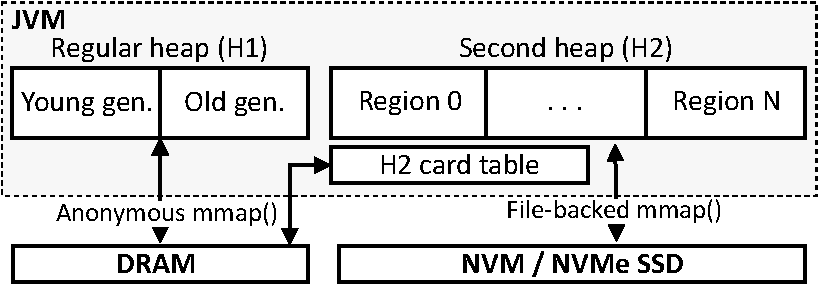
\includegraphics[width=0.6\linewidth]{teraheap/fig/teraheap_overview_a-crop.pdf}
  \caption{TeraHeap design overview.}
	\label{fig:teraheap}
\end{figure}

\paragraph{\textbf{How to prevent reclamation of backward references
(H2 to H1)?}}
Fencing \teraheapGC scans in H2 further requires tracking backward references
from H2 to H1, as the garbage collector must not reclaim H1 objects
referenced by live H2 objects. The key difficulty is that H2 objects
can reference objects in both generations of H1 and need to be tracked
differently. Young objects in H1 change location during minor \teraheapGC,
while old objects move only during major \teraheapGC. Scanning H2 to identify
backward references may incur significant overhead, depending on the
size of H2 and its backing device. Instead, we use an extended card
table for H2 to track backward references, optimized for
storage-backed heaps (\S\ref{sec:back_ref}).

Next we discuss how \teraheapName{} solves the three main challenges related
to:
%
(1) identifying and moving candidate objects to H2,
%
(2) reclaiming dead objects in H2 without \teraheapGC scans and I/O traffic,
and
%
(3) tracking backward references (H2 to H1) with low \teraheapGC cost and I/O
overhead.
